%% Copernicus Publications - AGILE-GISS Template for LaTeX Manuscript Preparation
%% ---------------------------------
%% This template should be used for copernicus-agile.cls
%% The class file together with some style files and the fontawesome5 package (optional use of the orcid iD icon) are bundled in the AGILE LaTeX template package.
%% For further assistance please refer to the AGILE web site (respective Conference subpages) at:
%% https://agile-online.org/

%% 2-column AGILE papers, please don't edit the following line
\documentclass[agile, final]{copernicus-agile}

%% \usepackage commands included in the copernicus-agile.cls:
%\usepackage[german, english]{babel}
%\usepackage{tabularx}
%\usepackage{cancel}
%\usepackage{multirow}
%\usepackage{supertabular}
%\usepackage{algorithmic}
%\usepackage{algorithm}
%\usepackage{amsthm}
%\usepackage{float}
%\usepackage{subfig}
%\usepackage{rotating}
\usepackage{hyperref}
%\usepackage{fontawesome5} %required to display the ORCID iD icon
\usepackage{enumitem}
\usepackage{flushend}
\usepackage{balance}
\hypersetup{
    colorlinks=true,
    filecolor=magenta,
    urlcolor=blue,
    linkcolor=blue,
    citecolor=black,
    }
\linenumbers % Please keep commented for submission of final version/uncomment if line numbers should be displayed during document preparation

%%%%%%%%
% HEAD %
%%%%%%%%

\begin{document}

\title{Guidelines for the visually accessible display of public transport routing}

\Author[1,*]{Till}{Frankenbach}
\Author[1,*]{Nikolaos}{Kolaxidis}
\Author[1,*]{Clemens}{Langer}

\affil[1]{Affiliation: Institute of Geography, Heidelberg University, Heidelberg, Germany}
\affil[*]{These authors contributed equally to this work.}

\correspondence{Sven Lautenbach (\href{mailto:sven.lautenbach@uni-heidelberg.de}{sven.lautenbach@uni-heidelberg.de})}

\firstpage{1}

\maketitle

%%%%%%%%%%%%%%%%%%%%%%%
% ABSTRACT & KEYWORDS %
%%%%%%%%%%%%%%%%%%%%%%%

\begin{abstract}

This research project explores the domain of inclusive map communication, focusing primarily on the accessible visualization of information for displaying public transport routes. It unravels the complexity of map design principles to enhance spatial orientation and readability, keeping the design appealing while introducing concepts for better accessibility.

One notable finding is the notion of "good-enough design", which acknowledges the need for tailored accessibility solutions using options for customization. This approach takes into account the wide range of user requirements, addressing diverse needs within the confines of established guidelines and standards. Our study furthermore investigates the effectiveness of focused maps in simplifying map information to enhance map accessibility. Moreover, the combination of visual and textual route representations and their distinct advantages are elaborated.

Our findings are in line with established research and guidelines, emphasizing the crucial role of adapted usage of visual variables for users with visual impairments. We offer practical guidance to guarantee conformity to these standards across different map components. Dissimilar to generic directives, our methodology adopts a user-centered approach, fine-tuning suggestions using expert insights and previously published works. This approach aims to produce effective solutions that meet particular user requirements by building on the work of expert researchers in the different fields.

\keywords{Routing visualization, accessibility, guidelines, public transport routing}

\end{abstract}

%%%%%%%%%%%%%%%%
% INTRODUCTION %
%%%%%%%%%%%%%%%%

\introduction[Introduction]

According to the World Health Organization (WHO), 253 million people are currently directly affected by a visual impairment \citep{WHO2023}. Due to the aging of the world population and an increased share in untreated diseases, the number is expected to increase significantly \citep{WHO2019}. These impairments formulate individual and diverse challenges and will lead to a decreased quality of life without according adjustments \citep{WHO2019}.

In regard to mobility, the importance of usable and accessible public transportation information in visual form cannot be overstated, especially for individuals with visual impairments \citep{EngelEA2022, NeuschmidEA2012, Sennekamp2022}. In today’s digital age with the prevalence of maps and navigation routes as well as easier and more accessible travel all over the world, the need for inclusive and user-friendly routing services is rising.

There already are different guidelines for accessibility in the context of web accessibility and even guidelines for interactive maps \citep{W3C2012, W3C2023, MinnesotaIT2023}. Based on these guidelines, there have been studies conducted to assess specific recommendations for action for specific visual impairments, like color blindness by \citet{JennyKelso2007} or blindness and impaired vision by \citet{EngelEA2022}. However, the broad diversity of visual impairments and therefore diverse partially opposing requirements for displaying information call for adapted accessibility methods \citep{NeuschmidEA2012}. For example, for some users, larger symbols are necessary to read maps effectively due to their blurred or unfocused vision, but for others smaller symbols are necessary due to the restriction of their field of focus \citep{NeuschmidEA2012}. 

The biggest research gap in this case is the lack of scientific resources and guidelines for making the public transport routing services accessible, especially in an interactive format. This gap highlights the need for evidence-based guidelines that include both areas of imaging and accessibility methods, ensuring that all users can access public transport with confidence.

Nevertheless, drafting a best practice, combining as many recommendations for action as proposed by different authors and institutions cannot suffice for the broad audience and would make interactive routing services even less accessible due to the high number of different visualizations. Thus, certain features should not be directly presented, but rather accessible "on demand". This means that developers should provide a tool set of customization options to personalize the routing service for the specific needs of the users. 

To address said research gap, we conducted qualitative expert interviews to validate our proposed guidelines for real-world application, focusing on practicality and efficacy. This paper provides practical guidelines for creating public transportation information that is not only visually attractive but also accessible to visually impaired individuals. We examine the concepts of "user-centered design", "good-enough design", the challenges posed by various visual impairments, the resulting user requirements for displaying routing information and finally the importance of complying with established web accessibility standards, but adapting them using new and established approaches and concepts.

This paper aims to summarize and introduce approaches and concepts that must be considered when developing visually accessible routing services from a user-centered perspective. Therefore, a fundamental basis in understanding the needs of different visual impairments and adaptable elements in routing services is elaborated.  

%%%%%%%%%%%%%%%%%%%%%%%%%%%%%%%%%%%%%%%%%%%
% STATE OF THE ART/THEORETICAL BACKGROUND %
%%%%%%%%%%%%%%%%%%%%%%%%%%%%%%%%%%%%%%%%%%%

\section{State of the art}

\subsection{User-centered Design}

User-centered Design is a methodological and conceptual framework within the domain of human-computer interaction and design theory. This approach is based on the systematic integration and evaluation of user needs, preferences, and experiences throughout the design process, seeking to ensure that the resulting product or service aligns with the specified user requirements \citep{KinzieEA2002}.

In user-centered design, design decisions and iterations are driven by empirical data gathered through several qualitative and quantitative methods, including the assessment of user needs or usability tests. The user-centered design process has an iterative nature, where assessments of user feedback are constantly reintegrated into the design prototype \citep{KinzieEA2002}.

As highlighted by \citet{ChammasEA2015}, technical standards and guidelines governing software-design have often been tested, evaluated, and applied in isolation from each other. In contrast, the user-centered design approach evaluates the interactions of multiple design choices and guidelines for each iteration. 

People with a visual impairment show a different set of user requirements resulting out of a diverging set of mental models applied in daily tasks \citep{Sanchez2008}. Therefore, accessible design approaches should take these into consideration from the beginning to result in a product that is both suited for users without disabilities and users with a range of diverse impairments \citep{RastovacEA2018}. 

\subsection{Visual impairments}

\begin{figure*}[t]
  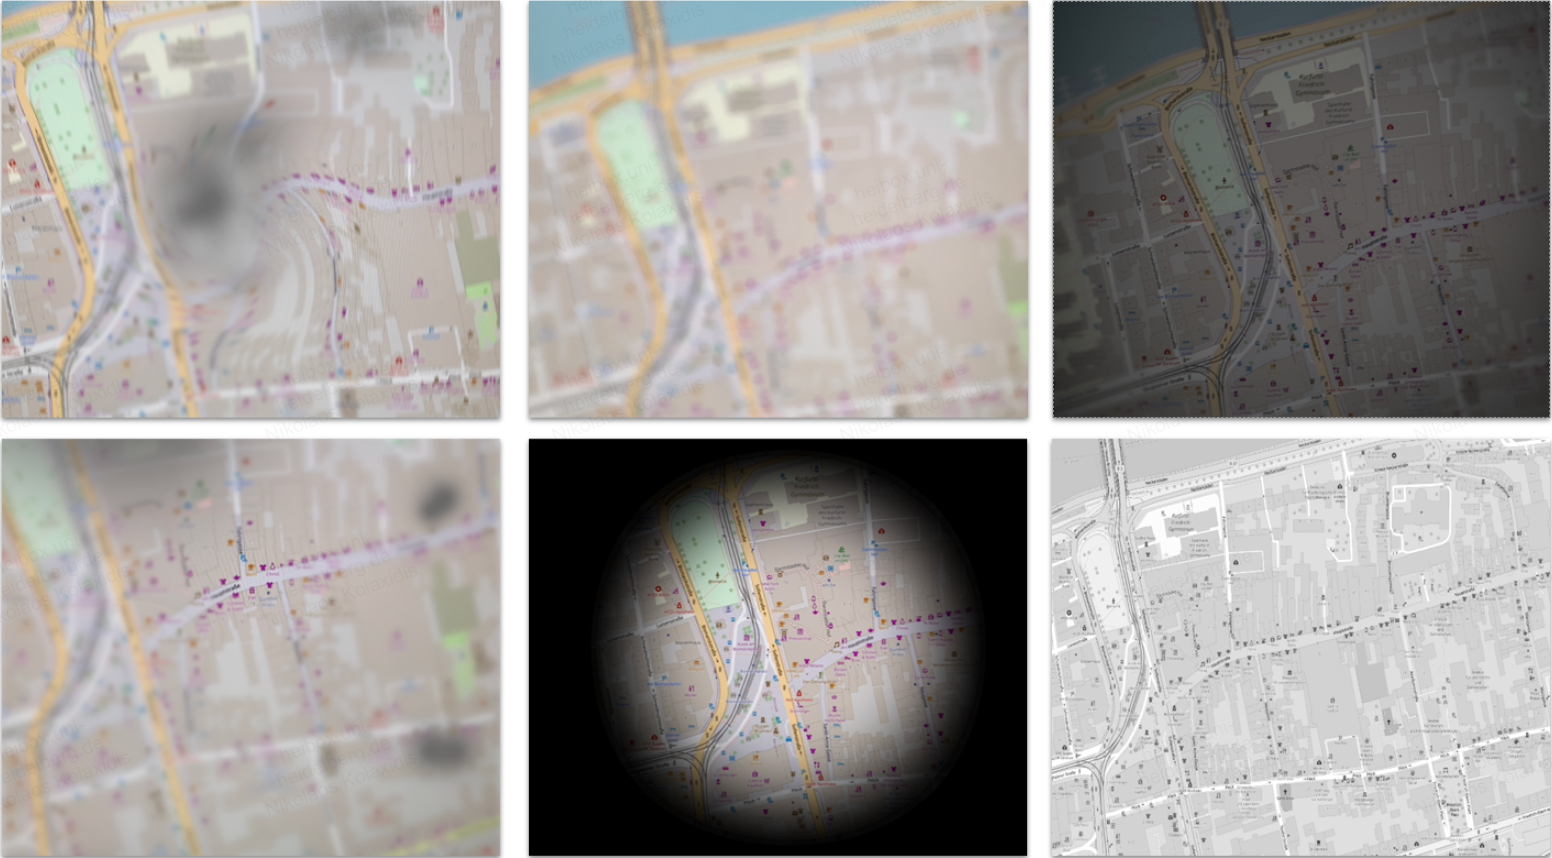
\includegraphics[width=\textwidth]{figures/visual impairments.png}
\caption{Different visual impairments shown exemplarily in a map view context. From upper left to lower right: Diabetic Macular Edema, Presbyopia, Retinitis pigmentosa, Retinal Branch Vein Occlusion, Glaucoma, Monochromacy representing color blindness in general. Captured with the ViaOpta Simulator app by Novartis Pharmaceuticals Corporation\textsuperscript{\ref{fn:viaopta}}.}
\label{pic:visual_impairments}
\end{figure*}

To better understand the challenges of end-users with visual impairments, it is required to take a closer look at the spectrum of visual impairments and the diverse symptoms in which they result.

Visual impairments include many conditions, each with unique visual challenges which influence the lives of those affected to various degrees. At the milder end of this spectrum, individuals may have partial vision. This means that even if they can see, their vision deteriorates, often leading to issues such as blurred vision or difficulty seeing fine details. These complications are often caused by conditions such as glaucoma, blood loss, or mistakes which cause a loss in visual acuity affecting the focusing of the eyes \citep{WHO2019}.

Moving onward in the spectrum, there are users with visual impairments. They struggle with, for example, highly reflective lenses, making tasks like reading conventional print or recognizing faces more difficult. This serious problem is due to progressive visual deterioration, where objects appear less clear and contrast decreases. Other potential symptoms include distortions in the viewing field (e.g. caused by Diabetic Macular Edema), blind spots (e.g. Retinis pigmentosa) or the loss of significant parts of the viewing field (e.g. by a progressed glaucoma) \citep{WHO2019}.  

At the opposite end of the spectrum, there are individuals with total blindness. For these individuals, visual information is severely reduced or absent, thus requiring reliance on alternative sensory modalities such as touch and hearing for pointing and information gathering.

In addition to these basic categories, there is a special category called color blindness. Color blind people show difficulties perceiving certain colors accurately. The most common are yellow-green and blue-yellow blindness, affecting the ability to distinguish between these two contrasting colors \citep{JennyKelso2007, NEI2023}.

In figure \ref{pic:visual_impairments} we exemplarily show the effects of selected visual impairments, demonstrated on the standard rendering of Open Street Map\footnote{\url{https://www.openstreetmap.org/}} (OSM). To simulate the effects, we used the ViaOpta Simulator app by Novartis Pharmaceuticals Corporation\footnote{\label{fn:viaopta}\url{https://play.google.com/store/apps/details?id=com.novartis.visionsimulator}} which can simulate different visual impairments using a mobile device.

Understanding this broad spectrum of visual impairments is critical to the development of mapping solutions that meet the needs of individuals with low vision. By considering these situations, we can create maps that are accessible and user-friendly.

A report by the \cite{WHO2023} underscores the global prevalence of visual impairment. In 2015, an estimated 253 million people worldwide were affected by visual impairment. Among them, 36 million individuals were classified as blind, and 217 million experienced moderate to severe visual impairment. Importantly, age plays a significant role, with approximately 80~\% of those affected falling into the 50 years or older age group. This highlights the growing issue of age-related vision problems and the importance of addressing the needs of older populations in eye care initiatives. Furthermore, it emphasizes the global scale of visual impairments and the urgency of accessible eye care services.

The research by \cite{AcklandEA2017} focuses on the demographic changes contributing to visual impairment. Over a 25-year period, from 1990 to 2015, the global population increased by 38 \%, from 5.3 billion to 7.3 billion. Moreover, the number of people aged 50 years and older nearly doubled, surging from 878 million to 1,640 million. These demographic shifts play a vital role in the increased absolute number of visually impaired individuals, despite other influencing factors. Understanding these trends is vital for developing targeted strategies and solutions to cater to the diverse needs of individuals with varying degrees of visual impairment, especially in a globally aging population.

\subsection{Guidelines for web accessibility}

Ensuring accessibility on the web is a major concern, and the World Wide Web Consortium (W3C) plays a key role in this effort. The W3C published the Web Content Accessibility Guidelines (WCAG), a comprehensive set of standards that provide a road map for making online content accessible \citep{W3C2023}. These guidelines point out some basic principles.

They emphasize the importance of things like font size, contrast, and distinguish-ability. These features are essential to make content appealing and readable, benefiting not only visually impaired individuals but also broader audiences.

The guidelines also point out that access extends beyond tangibles. It also includes performance, including keyboard access and compatibility with supporting technology. Ensuring that web interactions can be made through a keyboard and are compatible with screen readers and other supporting devices creates an inclusive digital environment.

In addition to the WCAG, the W3C developed the Accessible Rich Internet Applications (ARIA) specification, which provides a framework for increasing the accessibility of web applications. It allows developers to add semantic information to web content, making it more meaningful and suited for assistive technology. ARIA is especially valuable in communicating maps and ensuring they are accessible to visually impaired individuals.

The key principle of accessibility is a user-centered approach to design. Individuals with disabilities actively participate in the design and testing process. By engaging directly with the visually impaired, designers gain insight into their unique needs and preferences, resulting in more effective and inclusive mapping.

\subsection{Guidelines for web accessibility of interactive maps}

An article in the wiki of the W3C emphasizes the importance of ensuring that web maps are accessible not only to individuals with visual disabilities, but also to those with other diverse disabilities \citep{W3C2012}. The W3C provides a comprehensive resource that offers an overview of best practices for digital web maps. This includes incorporating proper heading hierarchy, logical navigation elements, and a clear reading order as fundamental for web map accessibility. Keyboard-based map navigation is stressed, along with providing alternative text and labels that adhere to color contrast guidelines. The guidelines further stress the importance of plain language usage and the inclusion of a comprehensive map legend. In addition to the topic of accessibility they offer an overview of various techniques  beyond the scope of visual representation.

The IT department of the state of Minnesota, USA, provides a summary of guidelines for interactive web map accessibility \citep{MinnesotaIT2023}, that align closely with the WCAG 2.1 and center their focus on ensuring web map accessibility for individuals with a wide range of disabilities additionally to the mentioned guidelines. These guidelines provide examples of effective methods to meet accessibility standards and emphasize the significance of accessibility in mapping applications. Practical examples for the implementation of proper heading hierarchy, logical navigation elements, and a clear reading order are highlighted, as these elements form the foundation of accessible web maps.

As mentioned previously, the assessment of user requirements is one of the key steps in the methodology of user centered design. \citet{EngelEA2022} have published the results of a questionnaire aiming to access these user requirements for way-finding and navigational tasks in unknown buildings for people with visual or mobility impairment. The included topics covered demographic data, experiences and skills, planning routes to unknown buildings, navigating in unknown buildings and experiences with building maps in general. While not every result is relevant for our research, we would like to highlight a few of the results. 

Many people affected by a visual impairment lack experience with using maps both in a physical and digital form. This highlights that an even larger emphasis must be put on the intuitive adaptation of offered web map services. Individuals with visual and mobility impairments have specific information needs when it comes to navigating unfamiliar environments. They require more detailed information about the places they intend to visit. This information is crucial for planning their trips and making informed decisions about how to reach their destinations within unfamiliar surroundings \citep{EngelEA2022,LoitschMuller2023}.

To plan their journeys effectively, individuals with impairments rely on various materials. These typically include digital maps, descriptions, and, for some, the assistance of companions or guides. Digital maps, accessible through interactive web applications, are particularly important, as they provide a visual representation of spaces and allow users to explore and prepare routes in advance. Additionally, text-based descriptions can offer valuable supplementary information for those who rely on screen readers or braille displays \citep{MelfiEA2022}.

While not directly related to web maps, \citet{ConstantinescuEA2022} explore the development of textual descriptions for indoor spaces to assist individuals with blindness. They underscore the critical role of detailed and clear textual descriptions, which, when integrated into mapping applications, can significantly enhance accessibility for individuals with diverse disabilities.

\citet{MelfiEA2022} introduce an innovative audio-tactile system designed to facilitate the exploration of indoor maps by visually impaired individuals. By offering alternative approaches for enhancing accessibility in mapping applications, this system paves the way for inclusiveness in geoinformation science.

\cite{LudersEA2022} outline adaptable indoor routing solutions tailored to the unique needs of people with disabilities. By focusing on broader solutions that emphasize inclusiveness and adaptability in navigation technologies, this research contributes to the overarching goal of ensuring accessible mapping applications.
 
\subsection{Visual variables}

Visual variables are the key concept for the visualization of geographical map data or, as in this case, the accessibility of interactive digital maps. They encode information using distinct visual properties of symbols and were originally described by French cartographer Jacques Bertin in his book \textit{Sémiologie Graphique} \citeyear{Bertin1967}.

He identified seven visual variables that can be manipulated to encode information, namely location, size, shape, color (including value and hue), orientation, and pattern or texture \citep{Bertin1967}. Bertin’s proposed set of visual variables was extended by \citet{Morrison1974} to include two additional variables used in cartographic design, the saturation of the color and the arrangement of symbol-intern visual elements. Finally, \citet{MacEachren1995} added another three visual variables, coming to a total of twelve, whose manipulation is made easier through modern digital production methods (formerly summarized under "focus"), namely crispness, resolution and transparency \citep{Roth2017}.

All these variables can be used to transfer information in a controlled manner from the map developer to the map user/reader. Usually, they are used for information graphics, of which maps can be a part of, rather than interactive applications \citep{NeuschmidEA2012}. Their ability to be associative and/or selective as well as differently scaled (nominal, ordinal, numerical) makes them flexible to use and gives them a very important role in the visualization of geographical information on maps \citep{Roth2017}. Therefore, in the context of routing visualizations, they must be considered a valid option to display specific information and direct the user's attention.

Nevertheless, routing services usually already use visual variables accordingly. In order to make them more accessible, these visual variables are not as vital as different new approaches in displaying them. Reusing established symbols and map elements but shifting their focus to accessible public transport routing using new approaches is more advisable than redeveloping them from scratch and redefining a whole new palette of elements. Consequently, these new concepts and the shift towards the accessible user-centered display of public transport routing are the key research topics this project focuses on. 

\subsection{Process of routing from the user's perspective}

\begin{figure*}[ht]
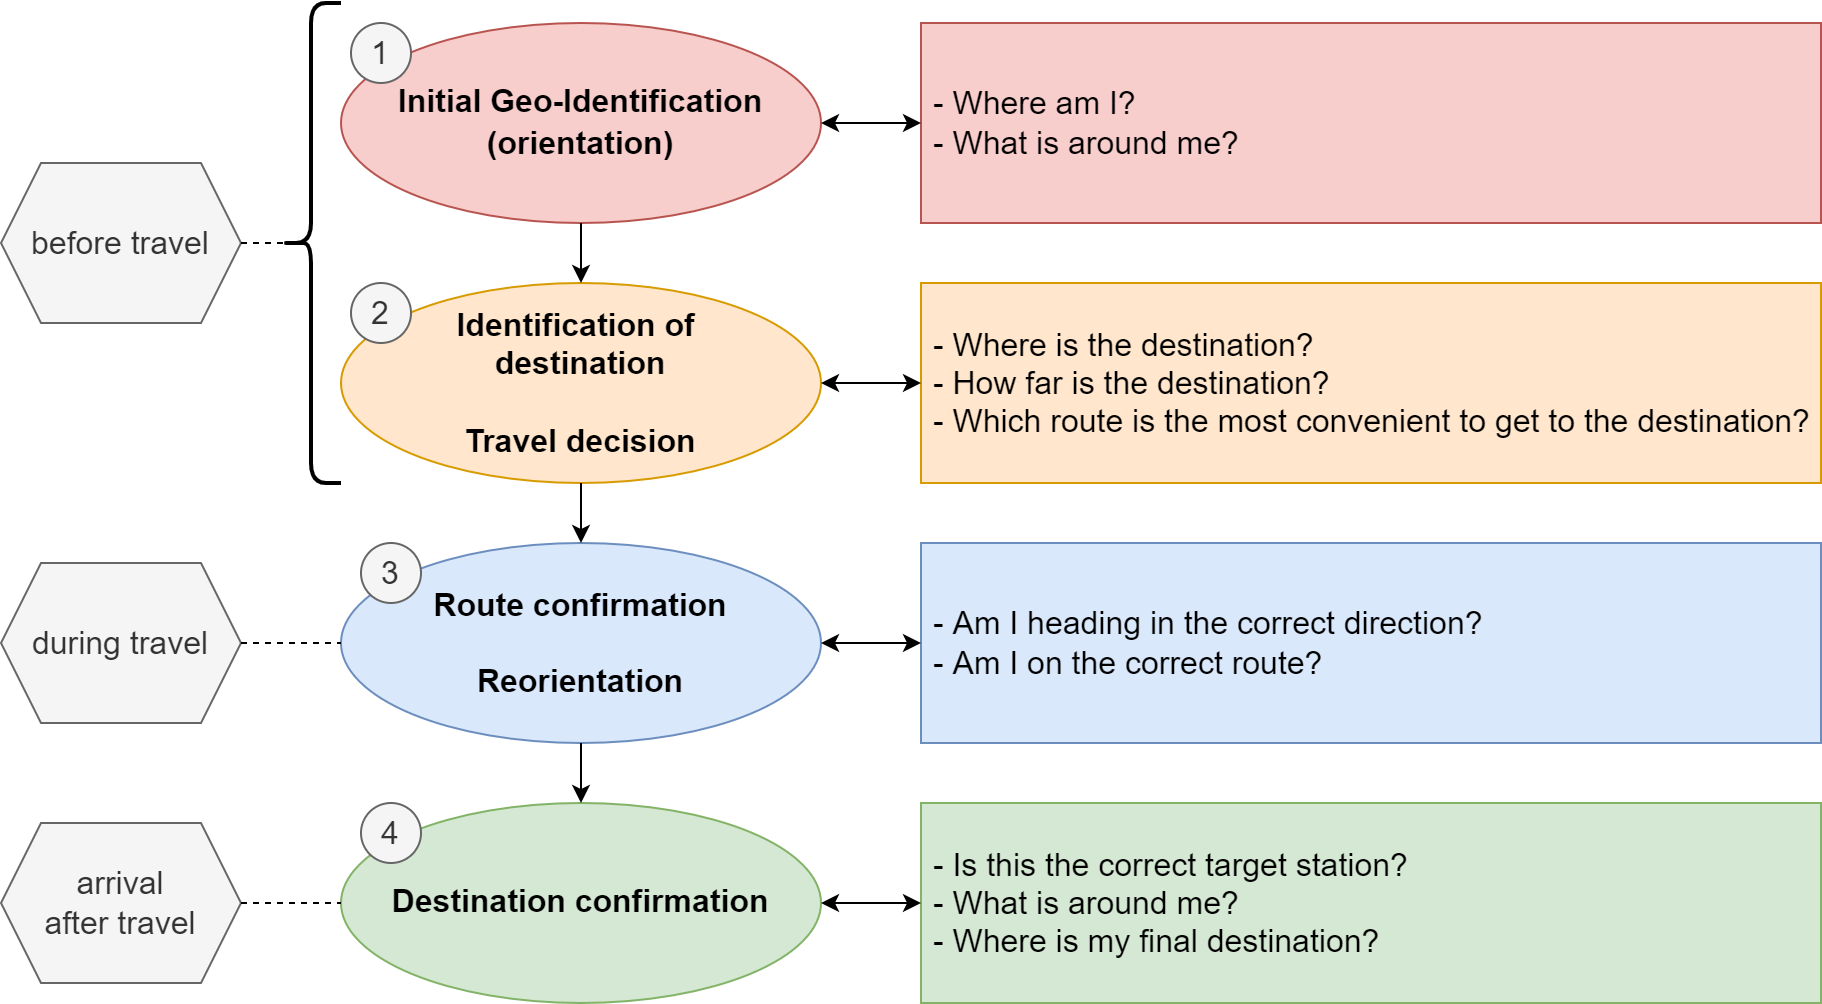
\includegraphics[width=\textwidth]{figures/route finding process.png}
\caption{Flow diagram showing the four main steps of the routing process from the user's perspective, including orientation and navigation tasks with related user questions. Adapted from \citet{Delikostidis2011}.}
\label{pic:route finding process}
\end{figure*}

According to \citet{Delikostidis2011} and as shown in figure \ref{pic:route finding process}, routing as seen from the user's perspective, therefore including route-finding and travelling, is a process consisting of four main phases. Each phase raises different questions and demands a variety of layers of information. In his explanations he even gives possible recommendations for action on how to display the information in order to possibly answer these questions, but due to the missing connection to public transport routing, some questions and recommendations for action are not suitable and are therefore adapted using further recommendations from \citet{Agrawala2002}, \citet{Zipf2002} and \citet{ZipfNeis2007} to better suit this topic.

\citet{Delikostidis2011} states that before the actual travel begins, finding a route starts by orienting in space and identifying the initial starting point as well as the destination. Questions here are of spatial nature, requiring landmarks and points of interest (POIs) which help finding specific points or addresses on the map, which itself should be shown as a well-known North-up overview. The importance of landmarks for the orientation process is further supported by \citet{ZipfNeis2007} in their work towards focus maps. Possible visualizations of landmarks in this context are shown by \citet{EliasEA2005}.

In order to choose the optimal and most suitable route, information like distance, duration, and properties of the route should be available to enable a comparison of different alternative routes. Regarding public transport routing, additional information about the modes of transportation and timetables should be accessible. This should be supported by depicting the route clearly in the same overview map along with start and destination points as well as landmarks to visualize the spatial properties of the route \citep{Delikostidis2011}.

After choosing a route and following it (point three in figure \ref{pic:route finding process}), constant reorientation and confirmation of the correct usage of transportation vehicles or roads requires other information than before, including names of stations, more detailed line information like numbers and directions and even changeover notices. Showing the current position can help provide suitable spatial information in close proximity to the route faster, which can enhance the route confirmation and reorientation processes \citep{Delikostidis2011}.

Finally, arriving at the target station has to be confirmed by acquiring information about the surroundings, directions, and possible further steps that have to be taken to arrive at the final destination, be it a point of interest, a shop, or other elements. Providing additional information like photos of places or descriptive text can make the destination confirmation more accurate, but is not strictly required \citep{Delikostidis2011}.

Additionally, \citet{Ormeling1996} introduces map use phases, in which different skills for different geographical questions raised during the routing process are required. For geographical questions regarding the "what?", users must be able to describe and identify certain elements, meaning that they should be distinguishable. Specifying and understanding the spatial position of elements ("where?") requires the classification, relation, and association of positions and elements, enabling the analysis of maps and their information. Further questions regarding contexts, transformations and developments require the interpretation of information, including explaining, predicting, and evaluating.

In order to offer specific information for the different questions and steps in the routing process, the map elements have to be shown selectively and precisely tailored for each demand. They can be adapted using the aforementioned visual variables summarized by \citet{Roth2017} and contextual visual aspects. All these different skills that are required to get all the information for each of the steps can be supported by adapting specific properties of route maps \citep{Delikostidis2011, AgrawalaStolte2000}. 

\subsection{Properties of route maps}

Regarding the process of routing from the user's perspective and its demands, \citet{AgrawalaStolte2000} summarize four primary objectives for the design of such route maps, namely readability, clarity, completeness and convenience. Readability is characterized by the easy and quick identification of all essential components of the route display, leading to a clear presentation with limited elements. Clarity aims at the unambiguous depiction of the route itself, accomplished by using appropriate symbols and line properties with an emphasis on minimizing superfluous details. Completeness prioritizes the display of all the necessary information required during each respective step in the routing process according to \citet{Delikostidis2011}. Going into more detail and concluding the goals, convenience is described as the need of considering the manner, timing, and context in which information is employed \citep{AgrawalaStolte2000}.

Central to these objectives is the principle to display only essential information. Additionally, information layers should adapt dynamically, displaying only vital information relevant to the current step of the routing process as introduced by \citet{Delikostidis2011}. Displaying too much information at once should be avoided at all times to keep the display of the route readable and clear as well as prevent the potential overcrowding of the display or, in other words, information overload \citep{AgrawalaStolte2000}. 

Additionally to displaying routes visually on the map area of the routing service, they can also be displayed via text, often found on the left side of the routing services in a separate area. These textual descriptions of the routes offer space for additional information regarding the route especially in the context of public transport routing, which otherwise would easily overload the visual representation of the routes. Therefore, the textual representation of the route must be considered as well with a similar principle.

Based on these design objectives, \citet{AgrawalaStolte2000} further introduced a framework of adaptable elements consisting of three variables, namely content, precision and rendering style, focusing, however, on the visual display of routes. 

Content describes fundamental map elements like starting and ending points along with reorientation points crucial for orientation \citep{Denis1997}. Contextual information further enriches content, and it comes in two primary forms. Local context includes path labels, street names, and landmarks such as buildings, bridges, and rivers. Landmarks are especially valuable for indicating orientation points and occasionally tracking progress along a road \citep{Denis1997}. Offering a broader perspective, overview context provides insight into the surrounding geographical area, aiding users in understanding how the route fits within its environment on a larger scale \citep{AgrawalaStolte2000}. 

Precision is vital for map accuracy. Due to the individual perception of the road network and landmarks, human-generated maps often feature distortions including inaccuracies in path lengths and road shapes \citep{Tversky1992}. By increasing the precision of the depiction, the route correlates more with the real world, but can potentially lessen the user-friendliness, especially in the context of public transport routing \citep{AgrawalaStolte2000}.

Rendering style comprises the aforementioned visual variables summarized by \citet{Roth2017} such as color value and hue, transparency, and line thickness (size) as well as contextual visual aspects like contrast and density of elements, affecting readability and clarity of a map. Choosing an appropriate rendering style helps users focus on important features of the map and interpret the map's relationship with the real world \citep{Agrawala2002, AgrawalaStolte2000, Sennekamp2022}.

In summary, content, including local and overview context, forms the map's information foundation, precision concerns controlled distortions or life-like depictions, and rendering style affects visual clarity. A successful map design involves skillfully balancing these variables regarding the four main objectives of route map generation and the visual variables. To aid the balancing, guidelines and recommendations for action should be accessible during the development process of the routing display, which, again, emphasizes the importance of this paper's aim, suggesting new approaches for the user-centered accessible display of map elements.

%%%%%%%%%%%
% METHODS %
%%%%%%%%%%%

\section{Methods}

The methodology of this research project encompasses the following steps: evaluating existing practices, collecting expert insights, summarizing recommendations for action, transforming them into visualizations to exemplarily show how they could be implemented into routing environments, and critically discussing the created elements regarding accessibility, appeal, and usefulness.

To establish a foundational understanding of the topic, an in-depth examination and comparison of current practices of different routing services was conducted, in particular: 
Google Maps\footnote{\url{https://www.google.com/maps}}, 
Bing Maps\footnote{\url{https://www.bing.com/maps/}}, 
Rome2Rio\footnote{\url{https://www.rome2rio.com}},
OpenRouteService\footnote{\url{https://maps.openrouteservice.org}} (ORS),
and, for specific display elements like the textual representation and additional symbol use,
the DB Navigator\footnote{\url{https://www.bahn.com/en/booking-information/db-navigator-app}} 
and Nav by ViaOpta\footnote{\url{https://play.google.com/store/apps/details?id=com.novartis.blind}} apps.
This involved identifying their respective advantages and disadvantages concerning the aforementioned main goals for route map design and the framework of adaptable elements presented by \citet{AgrawalaStolte2000} regarding the routing process proposed by \citet{Delikostidis2011}.

The specified points were discussed in three semi-structured interviews with experts in the fields graphic design, cartography, accessibility, community based research, and geoinformatics. Due to the broad knowledge and experience the interviewees offered, the interviews were planned as hour-long sessions with structured and specific questions as well as open questions asking for the spontaneous perception of elements from the experts' view.

The interview guide was split into two main parts which assessed the general appeal and perception of the routing services on the one hand and specific examples of good and bad practices based on the aforementioned goals and framework of such services on the other hand. The accumulated data gave valuable insight into the intersection of routing services, design, and accessibility, uncovering potential areas for improvement and possible best practices. It furthermore helped in enhancing directives extracted during literature review and developing a comprehensive framework for improving the overall appearance and perception of routing services as well as the visualization of routes and additional information associated with them.

In order to allow us to test the practicality and effectiveness of the proposed recommendations for action, the extracted guidelines were implemented within QGIS\footnote{\url{https://www.qgis.org/en/site/}}, in particular focusing on the ORS and its associated plugin\footnote{\url{https://plugins.qgis.org/plugins/ORStools/}}. This step facilitated the creation of visually appealing and user-friendly depictions of the routing services' proposed visualization and accessibility enhancements. These depictions also serve as potential recommendations for action.

Additional discussions where conducted with domain experts to assess the implemented guidelines and their impact on improving the accessibility to routing services, discussing the effectiveness of the proposed enhancements and their technical feasibility. Additionally, the recommendations for action were related to the aforementioned routing process and according questions raised during route finding to cover all steps and required information layers using multiple according recommendations for action. 

Through the systematic execution of these steps, this study aims to contribute to the advancement of perception of and accessibility in routing services, particularly within the realm of graphic design. The combined efforts of comparison of current practices, expert interviews, guideline extraction, practical implementation, and critical evaluation ensure a comprehensive and multifaceted exploration of the subject matter. Therefore, the main goal was to achieve improvements, uncover potential limitations, and gain suggestions for future research in this evolving field.

%%%%%%%%%%%
% RESULTS %
%%%%%%%%%%%

\section{Results}

The findings resulted from the consolidation of interview data while maintaining participant anonymity, supplemented with relevant literature findings to enrich the analysis. This approach adheres to ethical research standards by safeguarding the identities of interviewees and presenting an extensive comprehension based on existing literature. We recommended acknowledging the interdependent relationship among these data sources and emphasizing the significance of discretion, as well as the valuable knowledge obtained from related literature.

\subsection{Fundamentals}

There are general statements regarding the visualization of routes to make the services more appealing and accessible in addition to already existing guidelines from the OGC and W3C, which aim more towards interactive maps depicting data in general rather than routing services. 

One key recommendation for action is the visualization of information on demand as explained by \citet{NeuschmidEA2012}, \citet{AgrawalaStolte2000} and \citet{Delikostidis2011}. To avoid overloading the display visually, only the information required during the according step in the routing process should be shown. This complies with the introduced concept of "good-enough design", not implementing every type of visualization for all visual impairments and information levels, but rather offering an accessible base which can be individually adapted to the user's needs.

In addition to this, the routing should be target-group and application dependent, not showing modes of transport that are not requested. Information on demand can be achieved by using different levels of information which can be hidden and shown interactively. The interviewees mentioned that this concept of information on demand is the key advantage of digital media over static analogue media and should be used accordingly.

Regarding accessibility, another key concept building upon the potential of digital media is that most routing service elements should be automatically and manually scalable. First, automatically, to keep a clear display and prevent the element density on the map from overloading and elements from overlapping. As \citet{AgrawalaStolte2000} put it, focusing on the base map: "Roads should be variably scaled so that all roads and reorientation points are clearly visible and easily labeled". Second, manually to raise the adaptability to different visual impairment needs for both the visual as well as the textual route representation. 

Furthermore, developers should make use of a central geographical concept: Overview first, information second. Because, essentially, to appeal to the users and be useful, it should provide an overview of the position on the map and the different functions it offers first, and then display more specific information on demand.

Familiarity with and appeal of the routing service can be additionally enhanced by adhering to commonly known ("learned") visualizations to avoid confusing the map reader. These learned concepts represent the standards that the market leader (in this case Google Maps) has established. This can be the position of the textual representation on the left side or the dotted line style of footpaths, using outlines or shadow around the text or other elements of and in the routing service. Using such concepts not only creates a feeling of familiarity, but additionally makes the routing service easier to engage with. Nevertheless, these learned concepts can and should be altered and adapted to some extent to be more accessible for visually impaired users and fit more into the adapted routing service.

\subsection{Guidelines for the visual route representation}

Spatial orientation plays a big role in the routing process from a user's perspective. Therefore, "landmarks should be included where possible to denote the position of reorientation points and to communicate progression along the route" \citep{AgrawalaStolte2000}. Additionally, when routing, start and end points of the route should be clearly marked to emphasize and differentiate between start and destination.

Background maps were the first aspect mentioned by most interviewees. In this context, various factors contribute to a well-fitted base map. Firstly, the overall contrast of the map is crucial, as too much or too little contrast both result in additional time needed for orientation on the map during all the steps of the routing process (see figure \ref{fig:basemap_basic}). Additionally, excessive contrast draws attention away, making it more challenging for the viewer to focus on the depicted transportation route. Contrast should depend on the scale and increase with it to better distinguish differences of smaller objects on the map when looking, for example, at the footpaths. 

The experts recommend reducing saturation and lowering contrast with increasing scale (see figure \ref{fig:basemap_scale_contrast}). Footpaths should be depicted with high contrast to support orientation. Multiple base maps should be provided to choose from. Color pop or hue influence the order in which map elements are noticed, elements with high color pop being those noticed first. Only color palettes that are in line with accessibility recommendations based on color blindness by the OGC and W3C should be used. Different modes of transport should have different colors to make it possible to differentiate between them.

\begin{figure}[ht]
  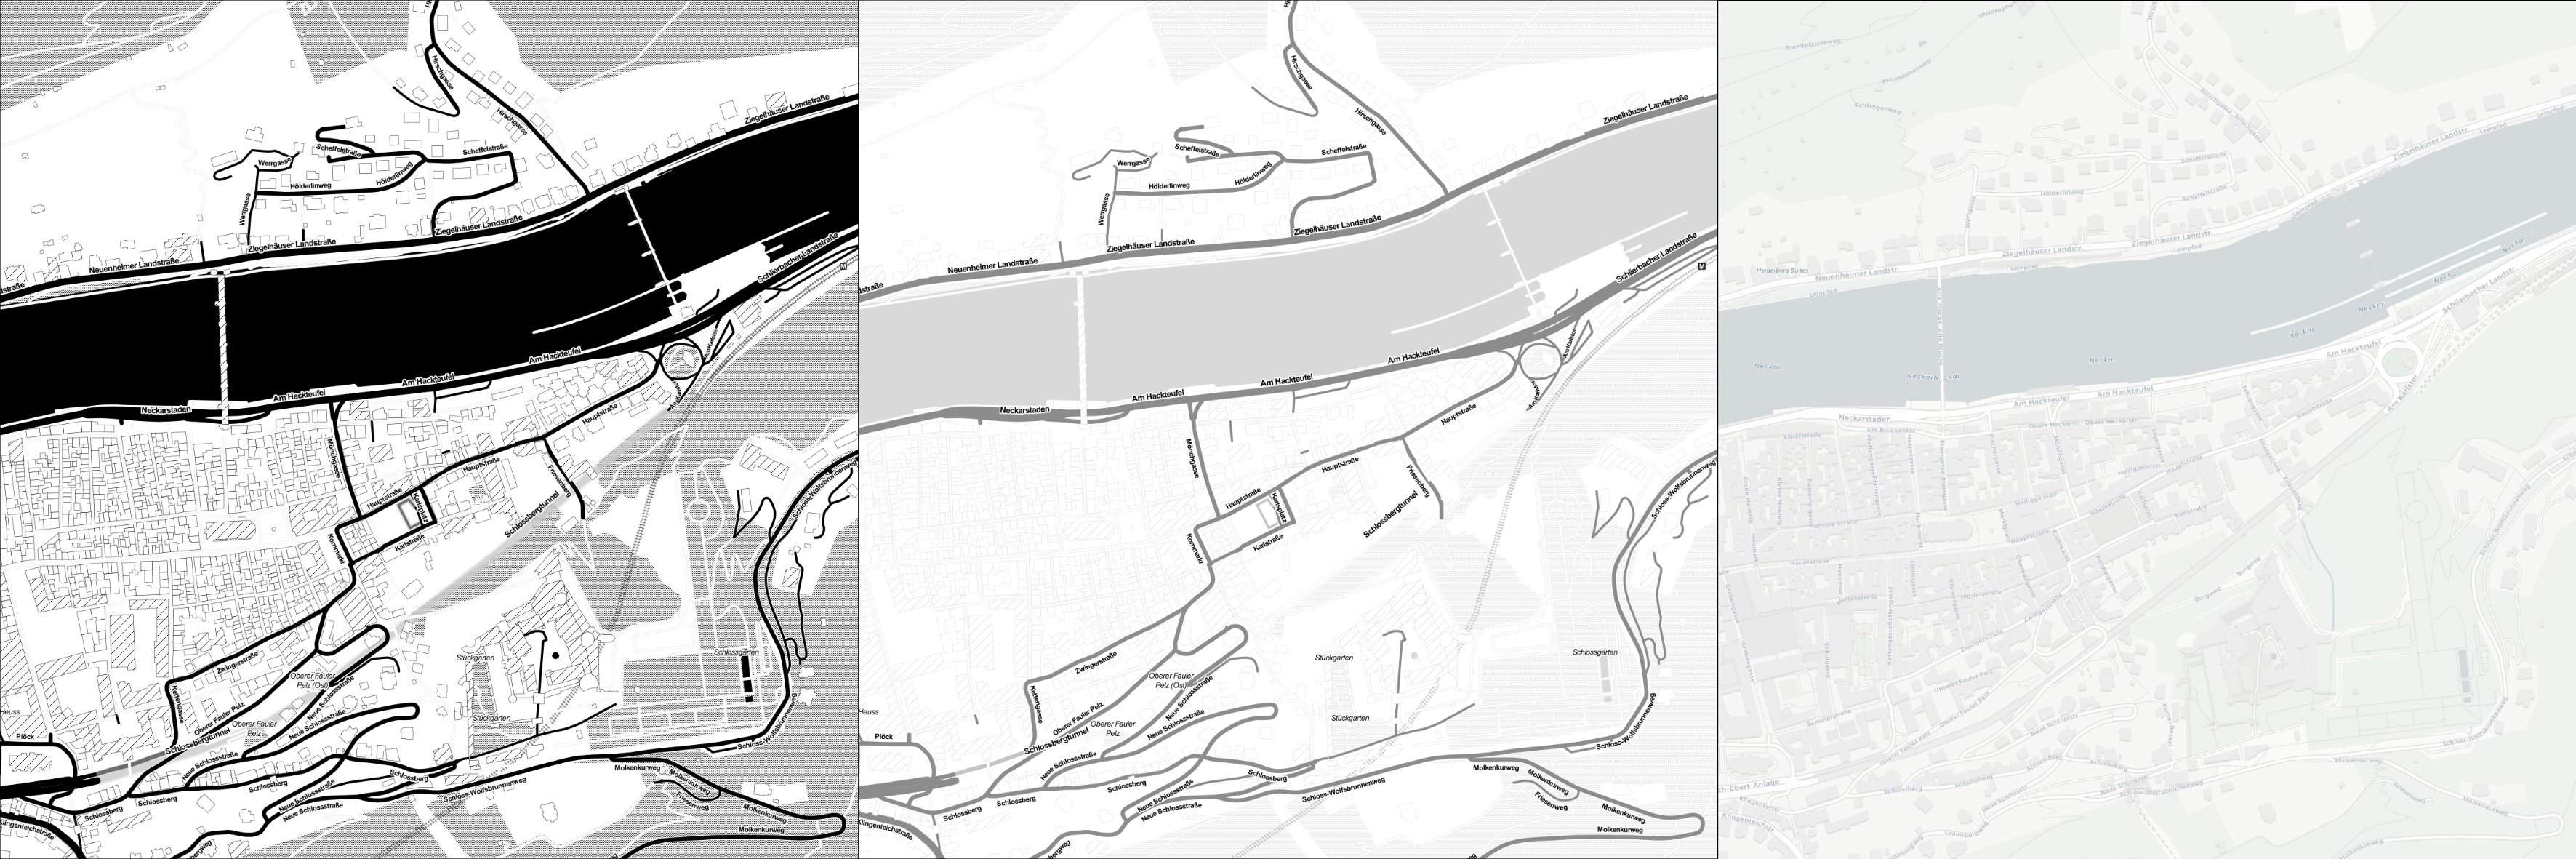
\includegraphics[width=8.2cm]{figures/basemap_basic.png}
\caption{Different contrasts to be used with base maps. Left: high contrast (Stamen Toner\footnotemark). Middle: lite contrast/grayscale (Stamen Toner Lite variant\footnotemark). Right: light color (CartoDB Positron\footnotemark).}
\label{fig:basemap_basic}
\end{figure}

\footnotetext[11]{\url{https://docs.stadiamaps.com/map-styles/stamen-toner/}}
\footnotetext[12]{\url{https://docs.stadiamaps.com/map-styles/stamen-toner/\#lite-variant}}
\footnotetext[13]{\url{https://github.com/openmaptiles/positron-gl-style}}

\begin{figure}[ht]
  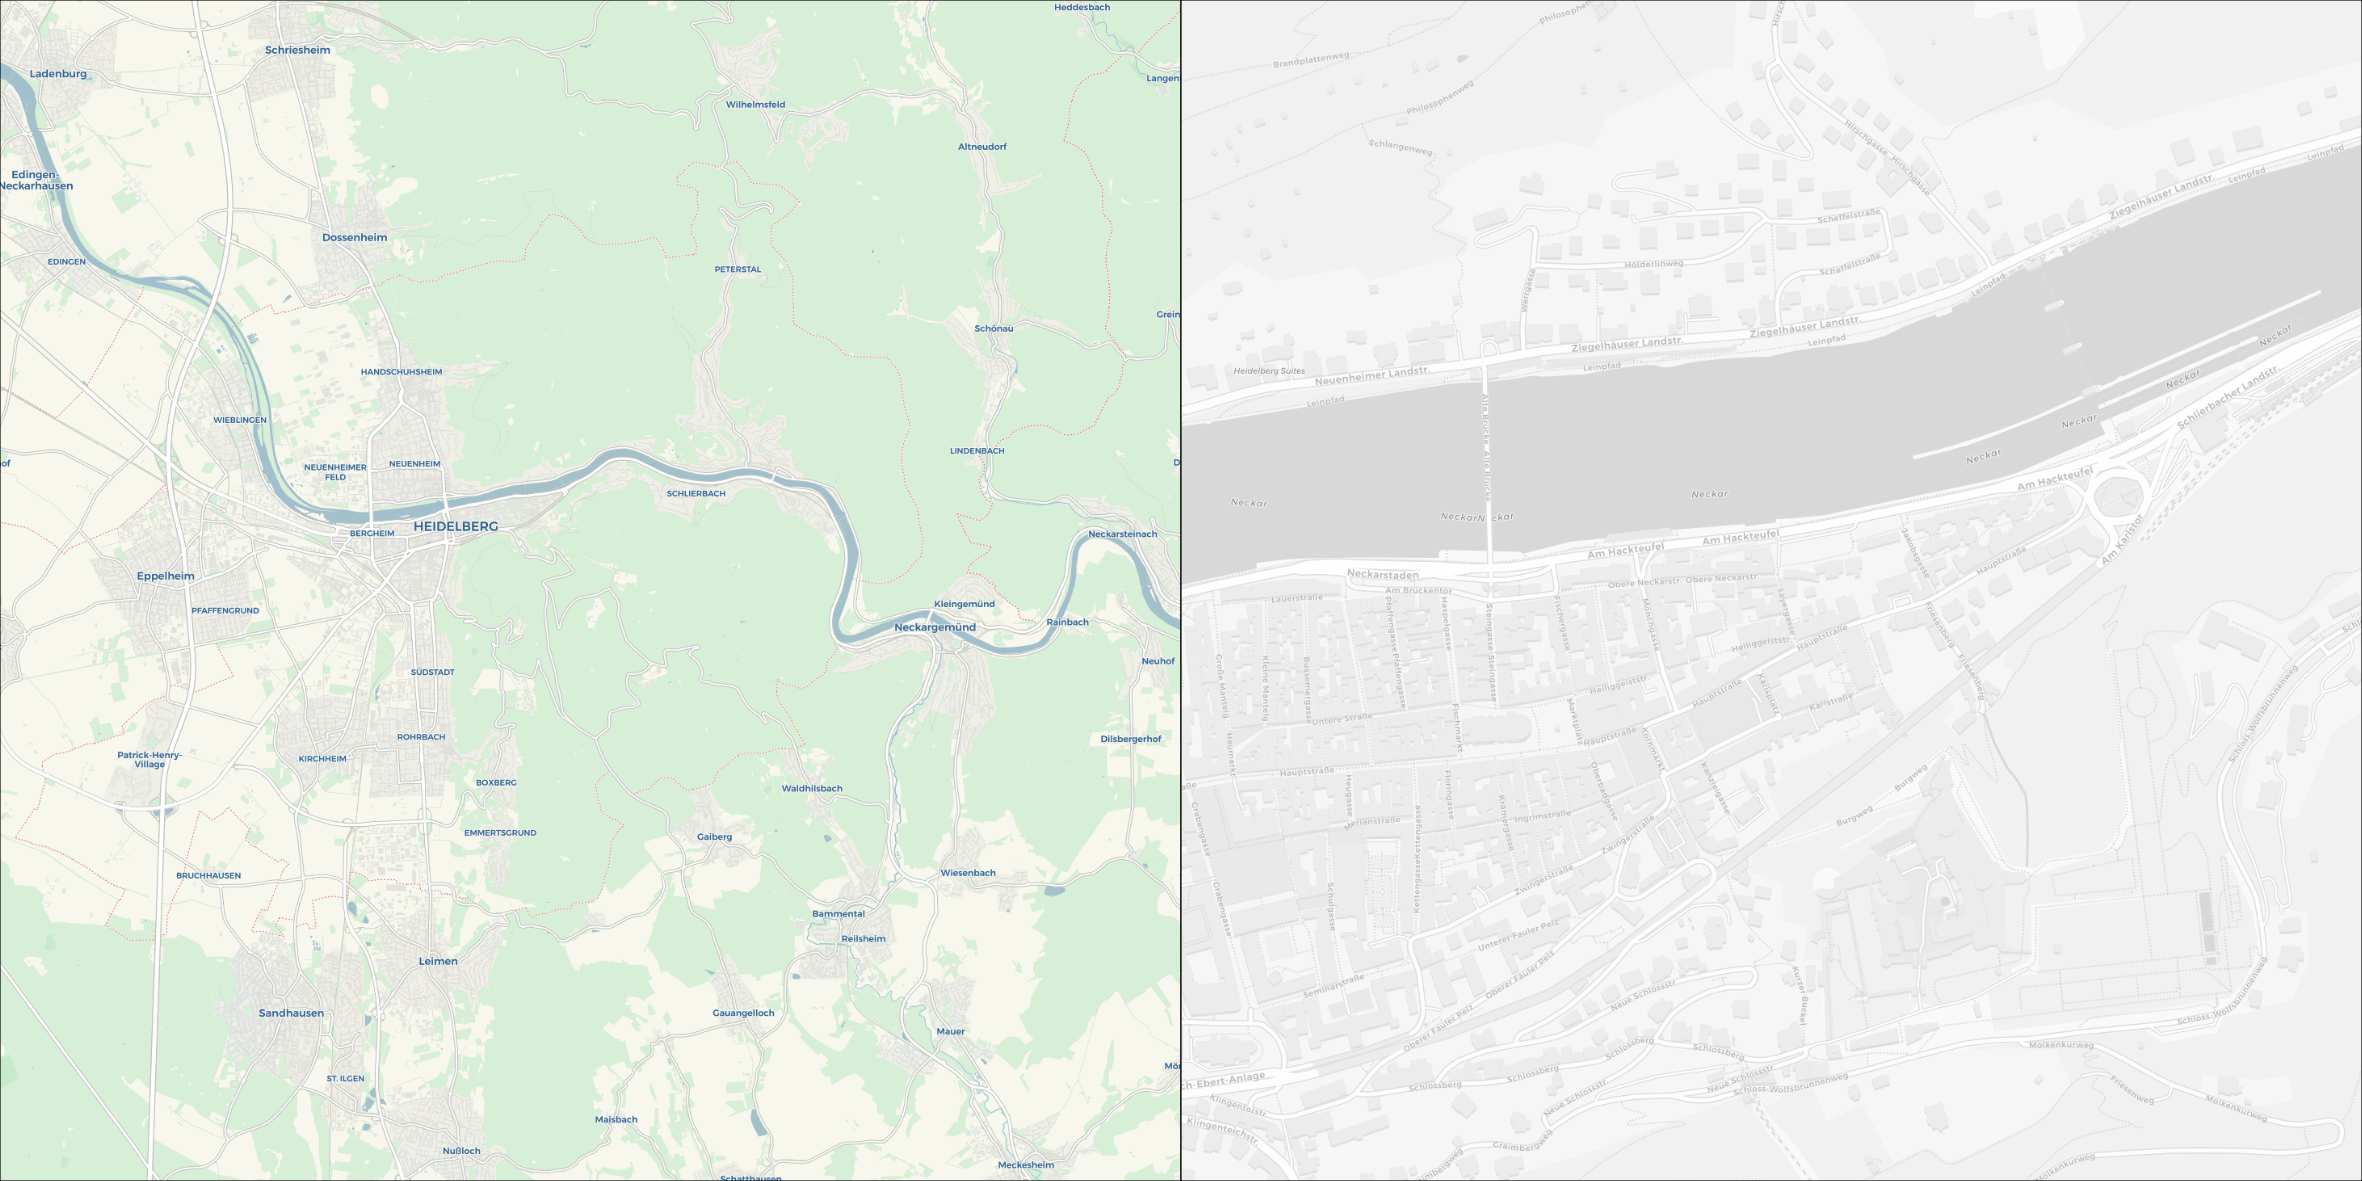
\includegraphics[width=8.2cm]{figures/basemap_scale_contrast.png}
\caption{Contrast and saturation at scale. Left: higher contrast and saturation at a low scale. Right: lower contrast and saturation at a high scale.}
\label{fig:basemap_scale_contrast}
\end{figure}

The concept of learned concepts as explained above applies to map symbols constructed with visual variables as well. For instance, commonly known pictograms for modes of transport should be used. Symbols should be used sparsely and with intention, their color should be adapted to their purpose (see figure \ref{fig:symbole}) and refer to the route colors. They should also be scalable on demand, allowing the visually impaired to optimize their size according to their needs. Only one or two patterns should be used. The pattern should be placed below the primary map information in the order list. Transparency can help keep the viewer from being overwhelmed. Dashed or dotted lines should not be used over opaque patterns to keep the perception clear.

\begin{figure}[ht]
  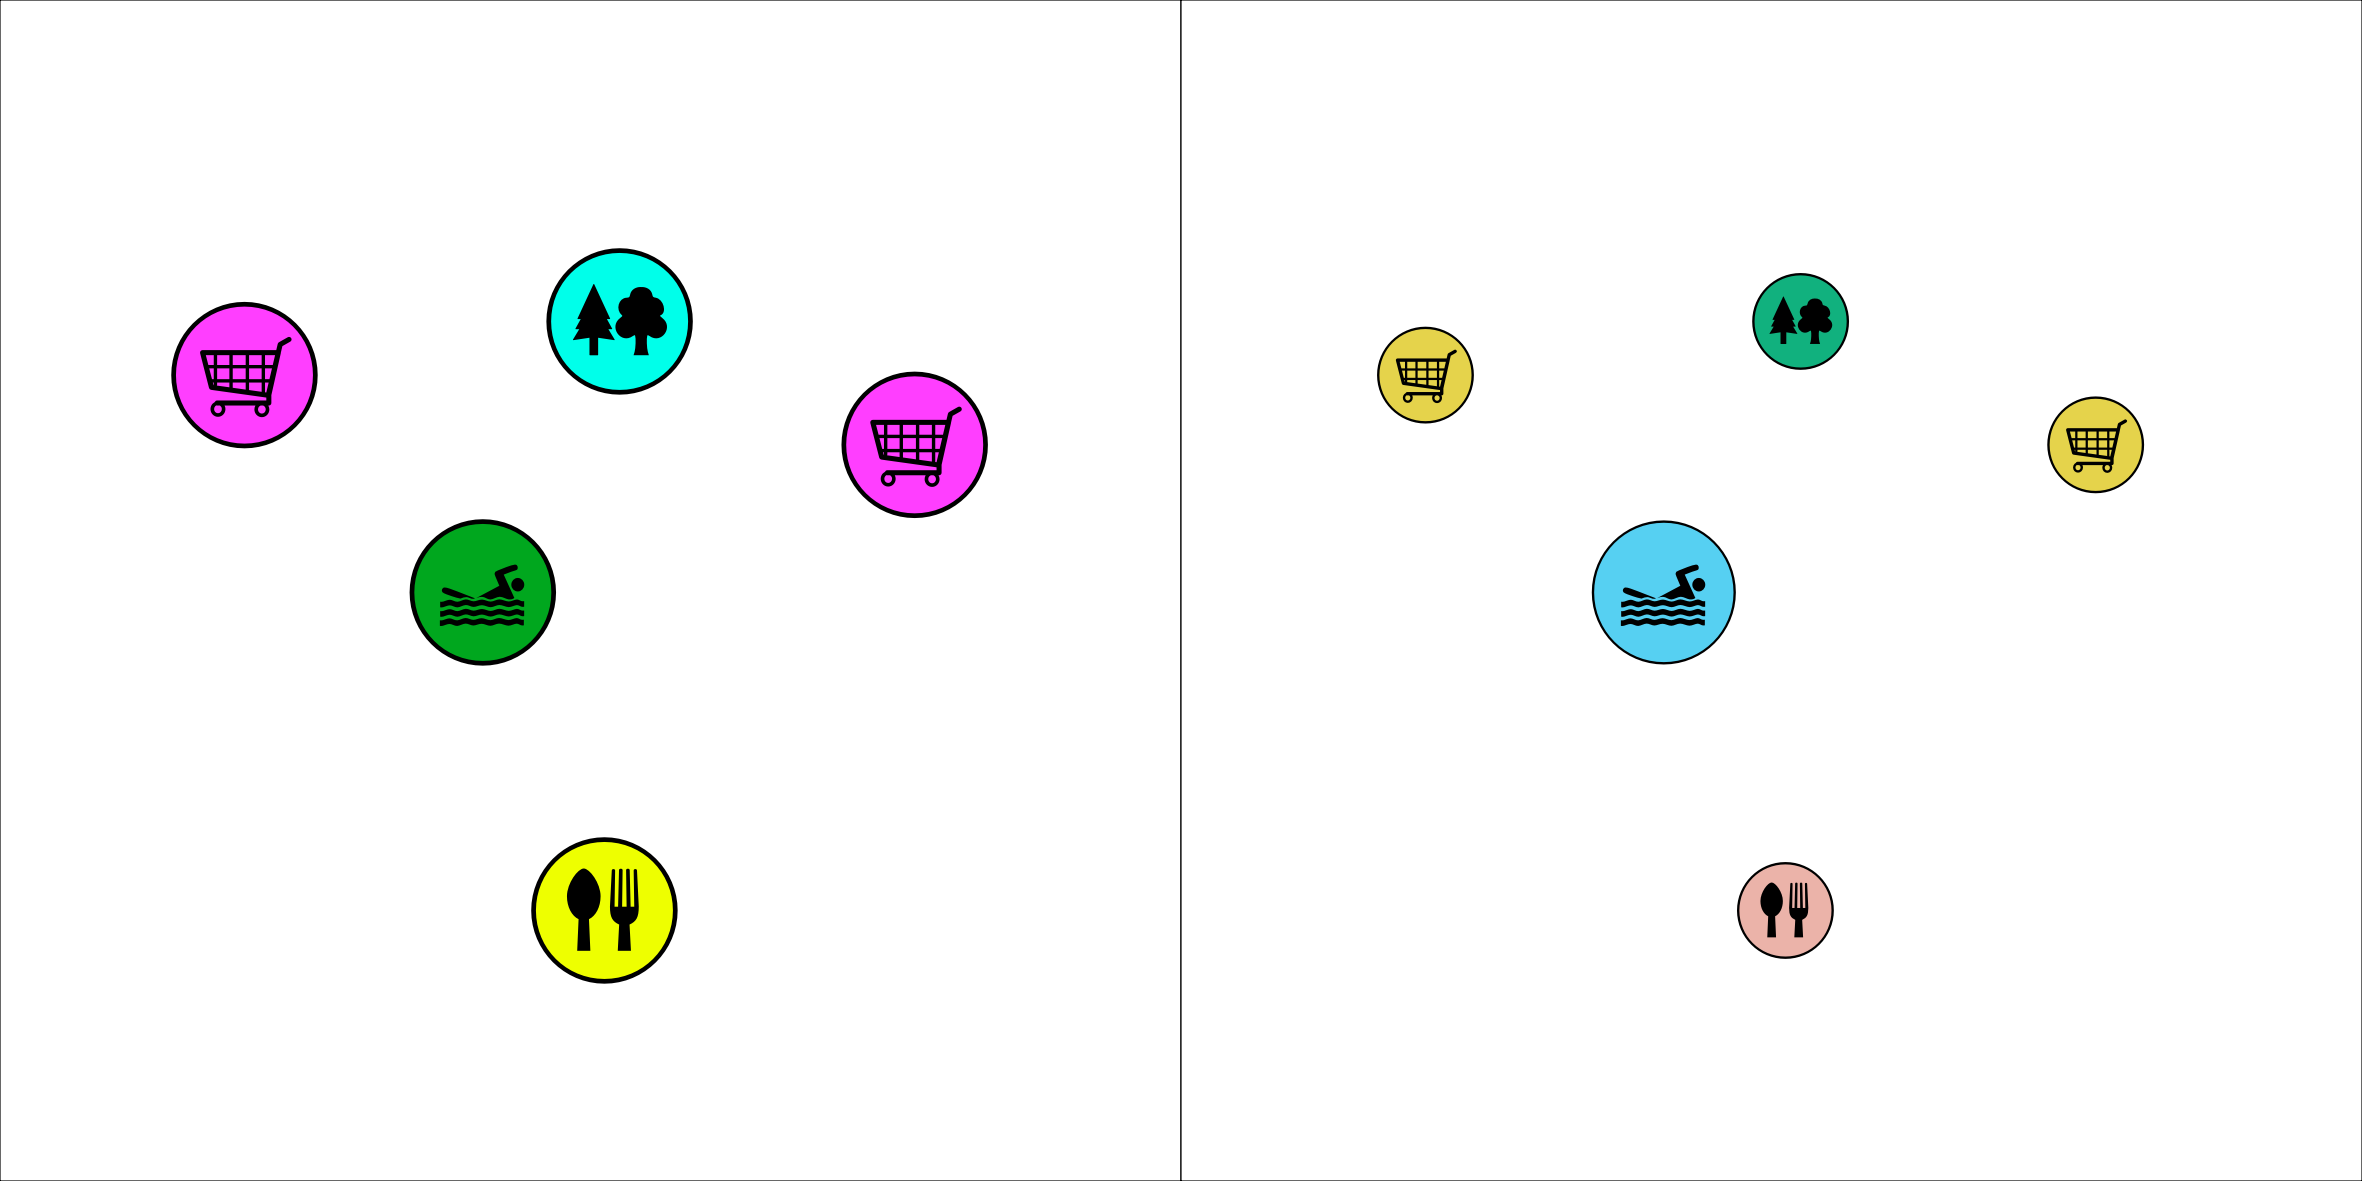
\includegraphics[width=8.2cm]{figures/symbole.png}
\caption{Use of color pop and relation in symbols (focus on swimming pool). Left (bad practice): colors do not match the depictions; the turquoise and pink symbols draw attention first due to color pop. Right (better practice): symbols do not draw attention due to color pop, different sizes, related colors for depictions.}
\label{fig:symbole}
\end{figure}

The styling of lines is another important consideration to be made. Bad representations include using colors present in the base map for the route itself, making it difficult to differentiate between map features and the route at first glance (see figure \ref{fig:linien_farbe}). Line thickness and outlines should be chosen carefully to ensure routes are quickly and easily recognizable. Thicker lines were recommended by the experts to improve map readability. Color assignment is important for distinguishing different route sections. Using the same color for walking and train routes, for instance, makes it difficult to determine where to get off the train and walk. 

\begin{figure}[ht]
  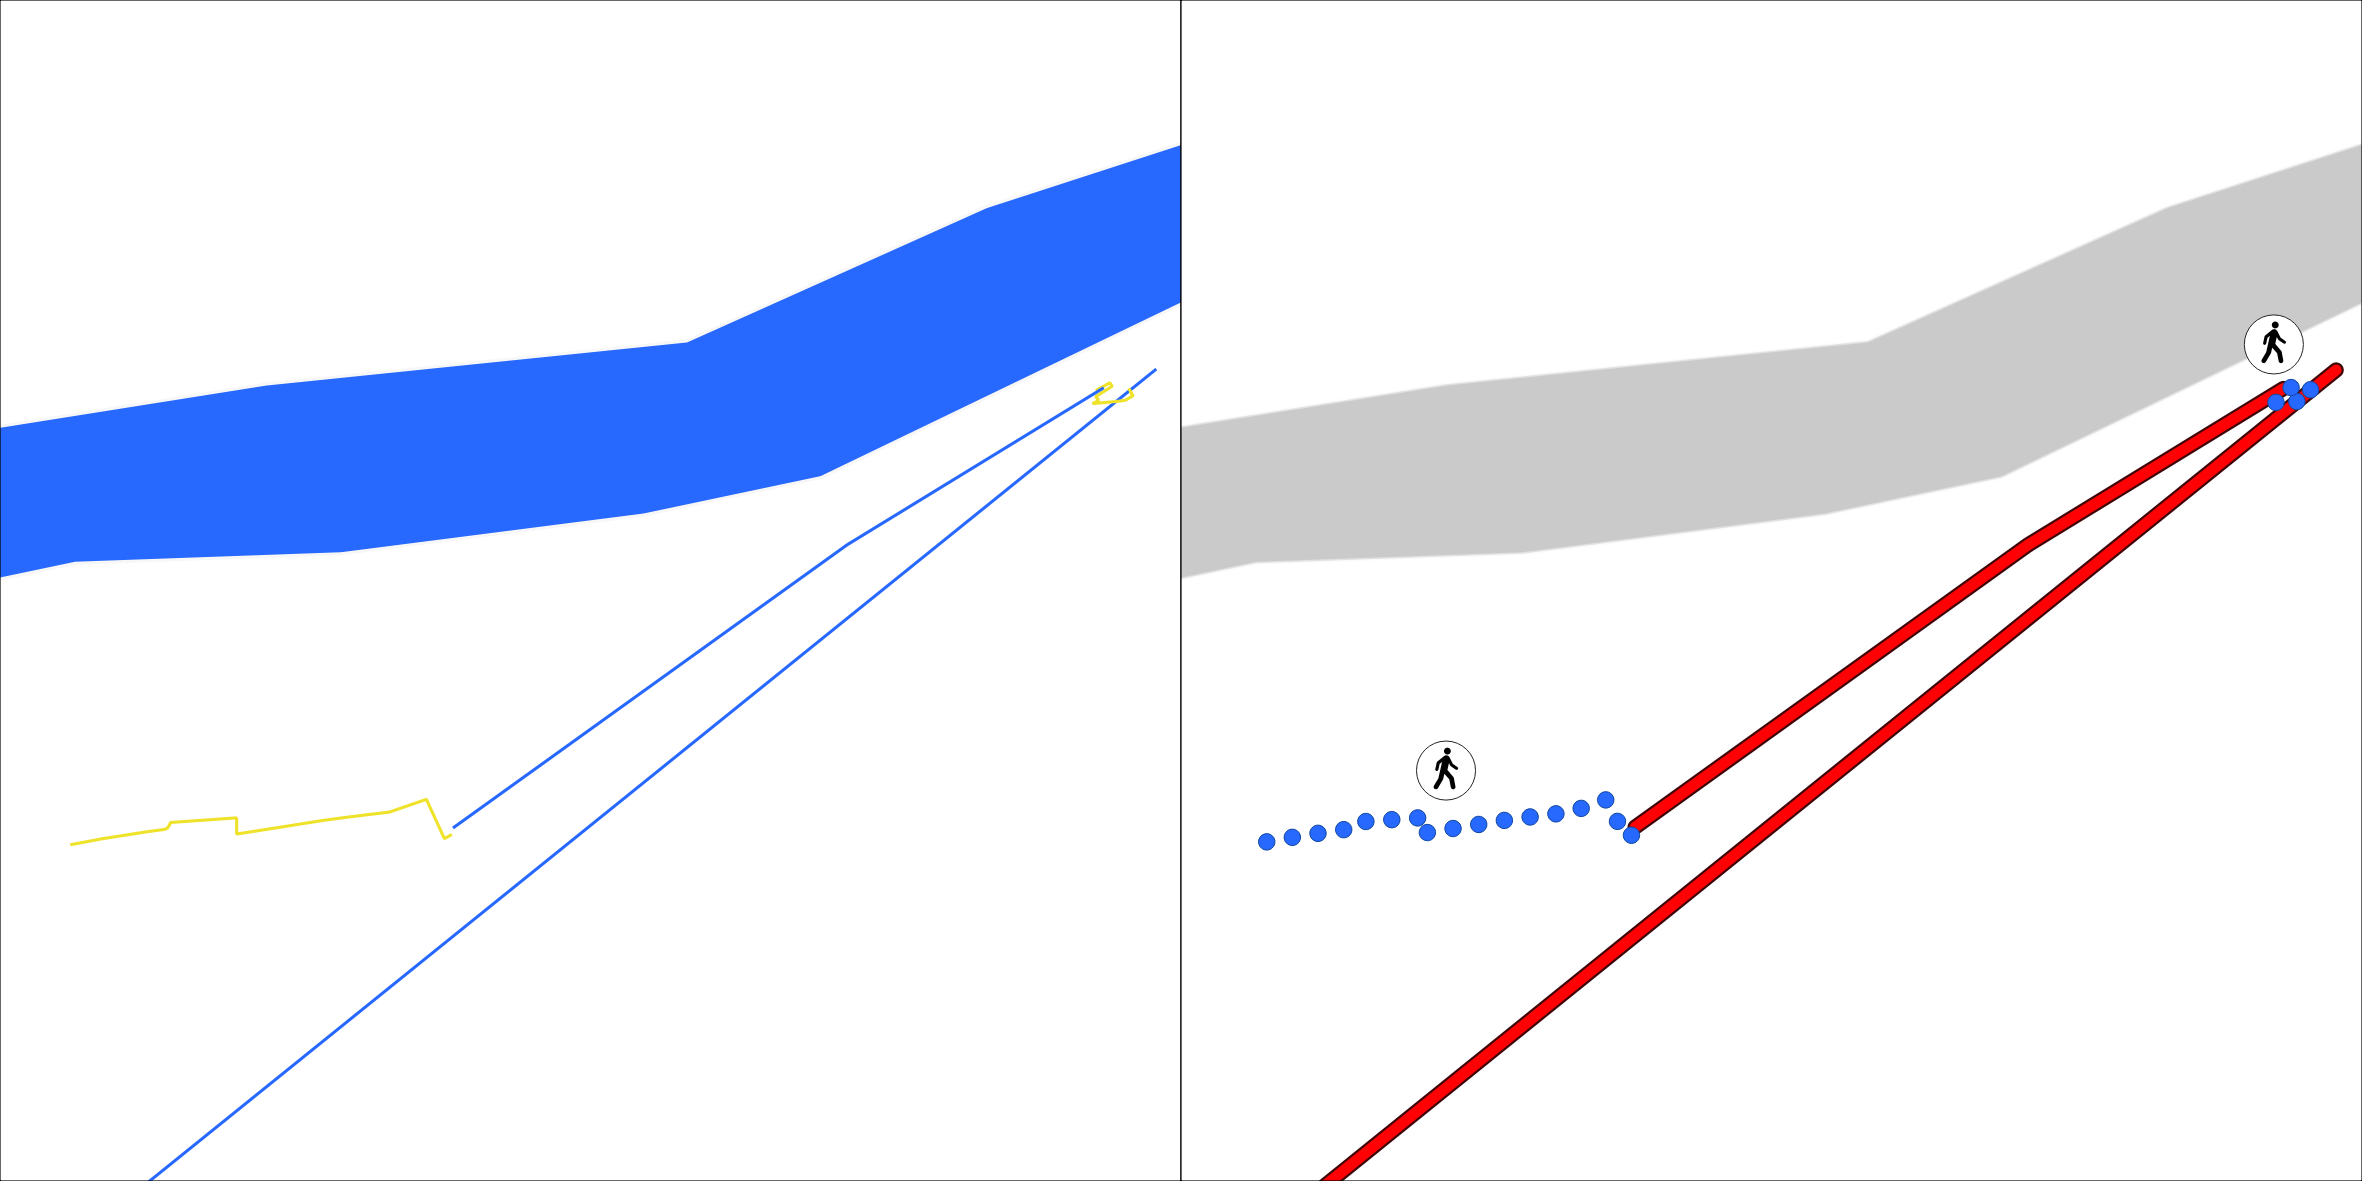
\includegraphics[width=8.2cm]{figures/linien_farbe.png}
\caption{Line styles in routing. Left (bad practice): potentially confusing color usage and bad line thickness. Right (better practice): thicker lines, distinguishable colors, and symbol usage for accessible clarification.}
\label{fig:linien_farbe}
\end{figure}

The font style can have typographical implications that must be considered. Adding buffers around the font can improve readability but may be less aesthetically pleasing from a design perspective (see figure \ref{fig:schrift} on the left). Most geographic information systems have a feature that allows text to follow the contour of the line to which it belongs. This approach facilitates fast reading and writing, but it is not typographically aesthetic as the letters have uneven spacing. From a design perspective the best font type is a simple straight font that has no buffer or shadow. This is shown in figure \ref{fig:schrift} on the right hand side.

\begin{figure}[ht]
  
\includegraphics[width=8.2cm]{figures/schrift.png}
\caption{Different font styles at curves. Left (bad practice): buffer and shadow around text. Middle (good practice according to cartographers): clear text following the curvature of the line for better relation. Right (good practice according to graphic designers): clear text without curvature for better readability.}
\label{fig:schrift}
\end{figure}

Another finding of the interviews is that any information on maps that is not important can be faded out. These focused maps reduce the depicted information in a map, making it easier to see information vital for the map's message. Previously researched by \citet{ZipfNeis2007} and \citet{ZipfRichter2002} and called "Focus Maps", the idea is to only display information valuable for the user. For example, regarding public transport routing, only POIs in a specific range around stations of the route should be shown, because other POIs (POIs which require longer stays) will not be of interest for the users during travel (see figure \ref{fig:linien_buffer_klein}). A QGIS feature called "Inverted-Polygons" is employed to achieve this.

\begin{figure}[ht]
  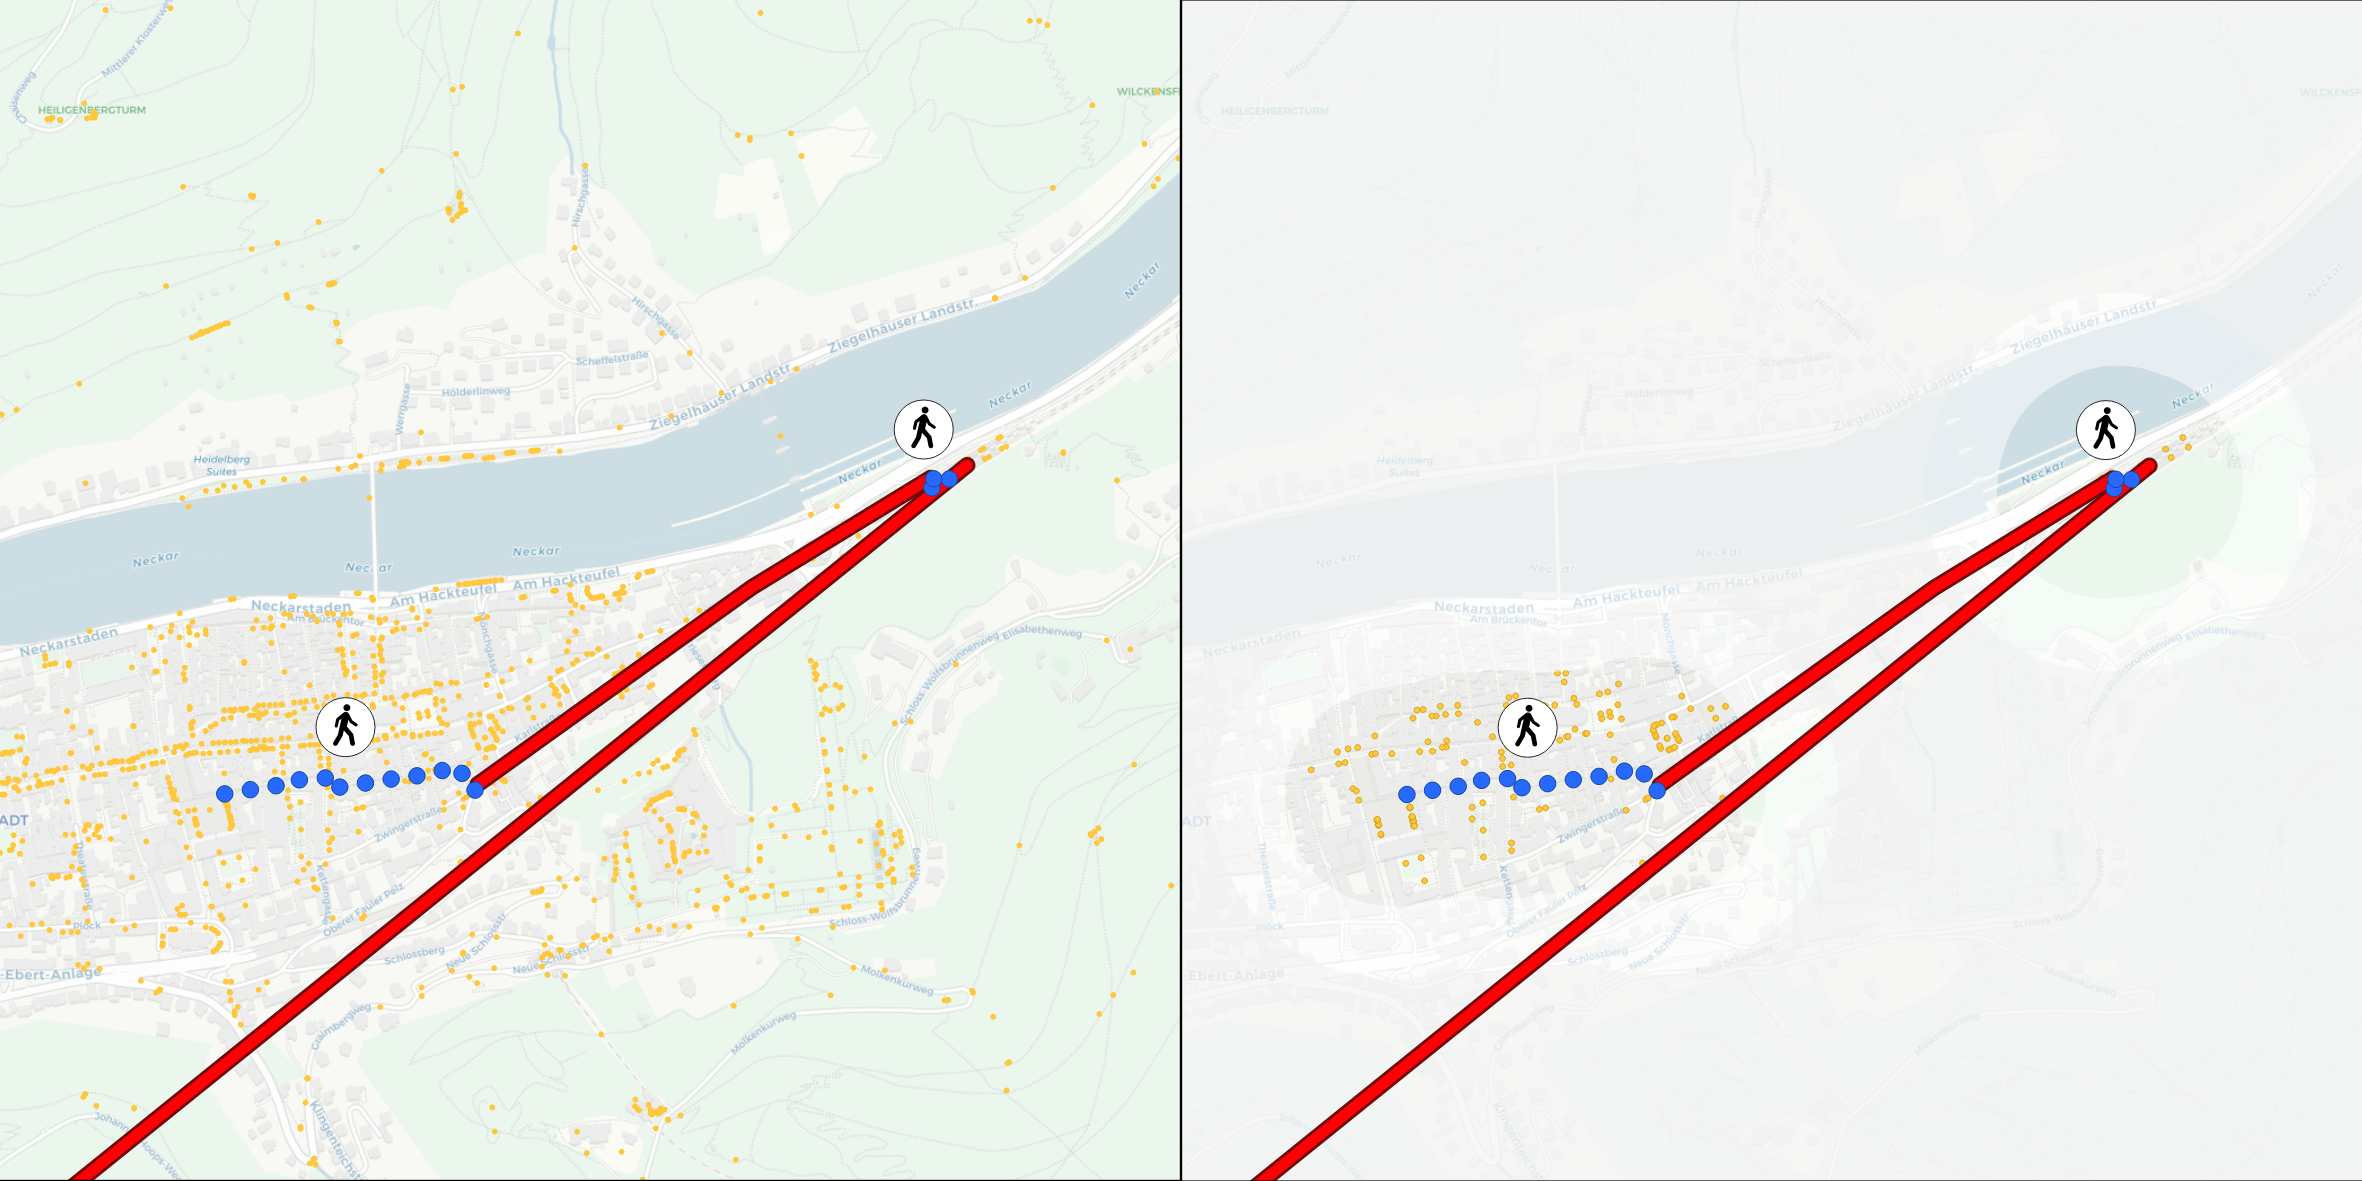
\includegraphics[width=8.2cm]{figures/linien_buffer_klein.png}
\caption{Focused mapping using the Inverted-Polygons method. Left (bad practice): many POIs in full view of the screen. Right (better practice): illustrative buffers around route with a selection of POIs which are accessible around the route during travel.}
\label{fig:linien_buffer_klein}
\end{figure}

Map-matching, a method to match geometries to a street or rail network, is not necessary for the visual representation. "The representation of a road [or rail] only needs to convey general curvature and the significant changes in orientation" \citep{AgrawalaStolte2000}. In public transport routing, further information on the modes of transport that have to be taken during travel are more important than the geometric precision of the driven routes. However, footpaths need a high geometric precision to be able to depict the correct route users have to use to get to the stations.

\subsection{Guidelines for the textual route representation}

As for the textual representation of the route, there are no specific recommendations available from the authors. In this case, the market leader in routing (Google Maps) and public transport routing (DB Navigator) should be used as a basis for further enhancements.

A first recommendation for action is to keep the text area separate from the map area using a bounding box with a different background color (mostly used: white). This ensures the user that there are two representations of the route and any visual overload is avoided. As most routing services have their textual representations on the left side of the windows, it is advisable to do so as well to generate a feeling of familiarity. 

Especially when showing different lines of public transport, the colors of the textual representation should match the colors of the map representation to visually match the according segments. Using this, the developers can use the textual representation as an additional information space for the visual route and vice versa. Interviewees criticized that Google Maps often shows the same route twice, both segmentally colored, as explained in the recommendation, as well as blue colored without distinction between line numbers and sometimes even with different duration specifications. This raises confusion and should be avoided. Bing Maps, in its current version, only provides single-colored routes on the map, but line colors in the textual representation, which is not appealing at all, emphasizing the importance of relating textual colors with map colors. 

The visual representation combines public transport routing and footpaths, which should be distinguishable as recommended above. Furthermore, additional information on the footpaths like length, duration and difficulty of the footpath using an elevation profile should be added in the text representation to give a basis for further considerations like finding an alternative footpath or using a bike for the segment. A similar approach is used by Google Maps and the ORS already when routing by bicycle, by foot, or by wheelchair, so the recommendation is to combine multiple routing algorithms. 

Another enhancement of the routing itself which would impact the text representation can be achieved by using wheelchair routing as it is already implemented by the ORS. A recommendation would be to use this routing for the footpaths before, during, and after the public transport routing for maximum accessibility on the route itself, but only if demanded so by the user. This should be accessible by a button in the text representation, not in the accessibility menu. The latter aims at making the service and front-end more accessible, not the route itself.

If using text-to-speech (TTS) services or so-called screen readers as suggested by \citet{NeuschmidEA2012}, the text should not be hidden in a drop-down menu, because in some cases the TTS software cannot open the menu to access the text. But as we focus on visually impaired and not blind users who would strictly require TTS software, drop-down menus are more appealing. They are used in current routing services and are a commonly used method of keeping the textual display clear.

In regard to step number three of the routing process according to \citet{Delikostidis2011}, route confirmation, a helpful method would be to show the names of the stations before and after a changeover in the textual representation along with the usual line numbers, travel direction, platforms, and mode of transport. Thereby, users will have more time before a changeover to prepare themselves and will have a type of quick confirmation that they took the correct public transport. Another useful addition would be the information if the users would have to change the street side during the changeover to avoid losing time during (re-)orientation.

The text area can provide useful additional information for the route. As for recommendations, keeping close to the market leaders and combining their practices but implementing some enhancements for increased accessibility and orientation is advisable. Overloading the text area should still be avoided. 

%%%%%%%%%%%%%%
% DISCUSSION %
%%%%%%%%%%%%%%

\section{Discussion}

The discussion is structured in multiple sections and puts the results into context after critically reflecting the used methodology. 

\subsection{Critical reflection of the methodology}

This research project focuses on the accessibility of routing services and aims at summarizing and introducing approaches and concepts that must be considered when developing visually accessible routing services from a user-centered perspective. Research questions include what elements have to be considered adaptable, which concepts and guidelines exist already and which new approaches are necessary to develop an accessible public routing service. The wording of those could be more concise. There are several reasons as to why this is the case. Firstly, the topic which this study is aimed at is a very broad one. For instance, one might jump to the conclusion that in a front-end for people with visual impairment, it would be the best approach to structure it in a way in which every user can choose their impairment and get exactly the depiction for their needs. In theory, this might look promising, in practice, however, it is simply not achievable. The spectrum of impairments is too broad and in itself not discrete. In turn, a simple depiction that fits the need of all is also impossible to achieve, since needs of the visually impaired diverge, regarding focus area and symbol size, for instance. The conclusion that most features should be on demand is a compromise. The same applies to the research questions. Putting the research in a broader context would have, in turn, resulted in more vague results. A more specific context allows for the possibility of overlooking generalities.

\subsubsection{User-centered design without the user}

As explained earlier, we have embedded our work in the context of a user-centered design process. Yet, this work only covers parts of this design model. Certain parts, as the assessment of user requirements for software products and interactive web map services in particular, have been previously published for example by \citet{NeuschmidEA2012}, \citet{Delikostidis2011}, \citet{EngelEA2022} and \citet{AgrawalaStolte2000}. The core of our methodology was to extend these by evaluating how present routing services might already meet such existing requirements and guidelines to extend those with the knowledge provided by the interviewed experts. 

Yet, this methodology neither involves an actual visually impaired person nor any other user testing to evaluate the proposed guidelines. Therefore, the provided results cannot be interpreted as final or universally applicable. They should rather be seen as a starting point for further research and aspects that must be considered during development of a routing service. This includes evaluating some of the proposed benefits in isolation, but also evaluating the interaction between various guidelines and proposed changes. 

\subsubsection{Interviews}

In this study, three interviews with a duration of around one hour were conducted with experts from varying fields. They covered the most important fields available in the time span in which the study was conducted. However, especially regarding user-centered design, more interviews should have been done to get more opinions and expertise from even more fields like information design, accessibility research in general, or front-end development. An interview duration of around one hour was chosen since it provided the best compromise between being able to process and transcribe all the interviews and gaining as much information as possible.

The semi-structured form of interviews was chosen, because it brings a high level of exchange between the interviewer and interviewee \citep{KallioEA2016}. Also, a fully structured approach would not have provided the necessary freedom for the interviewers to approach questions that arose during the interview itself. Conversely, an approach without any structure would have made it difficult to bring the attained results together and interpret them as one, especially when using a congruent basis like the routing process according to \citet{Delikostidis2011} and the route map properties introduced by \citet{AgrawalaStolte2000}.

\subsubsection{Chosen routing services}

The routing services used in this project are all prominent in the digital routing and maps industry. Although one may have initially perceived a bias towards larger companies before conducting interviews, our current perspective suggests this concern is baseless. The concept of common knowledge in form of learned visualizations introduced by the market leaders is important here. Taking smaller routing services into account which use a lot of different symbols, styles, and other elements, would have been counterproductive in this context. It should be noted that there may be valuable concepts offered by these services which were lost by not considering them. Nevertheless, given the study's scope and time frame, the chosen approach was likely the most appropriate one.

\subsection{Results}

Creating a full size visual representation with all gathered recommendations has not been done due to the time frame of the project and missing tools in the QGIS environment. This project focused on concepts and guidelines based on the idea of a "good-enough practice" rather than multiple specific best practices. Therefore, creating one example which could be interpreted as "best practice" would miss the central scope of this project. Additionally, routing services are interactive systems and when using the concept of information on demand as explained above, there cannot be only one specific depiction of an adaptable interactive visual representation; this would drastically miss the point.

However, as \citet{LoitschMuller2023} show in the first phase of the user journey map used in their study, there can be routing services offering multiple templates of individualization options for specific visual impairments. These can afterwards be customized and adapted to the user's needs using additional options. An idea to implement such customizable functions is an accessibility menu hidden behind a button with a commonly known pictogram depicting accessibility (see figure \ref{fig:accessicons}) as it is used for example by the ORS. The menu could contain sliders or multiple step selectors to change the line widths, contrasts, font or symbol sizes etc. of both the visual and textual representation.

\begin{figure}[ht]
  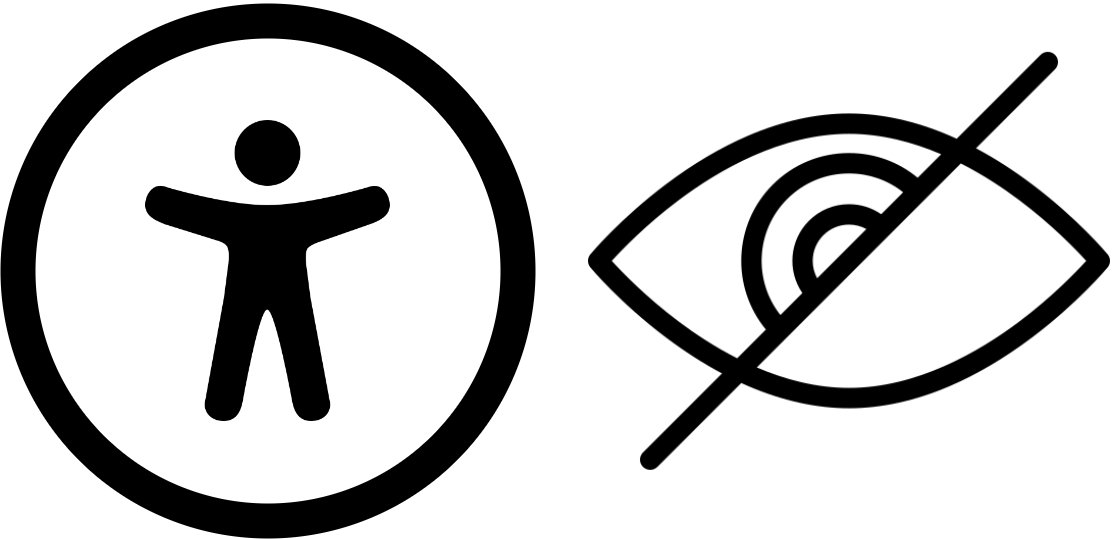
\includegraphics[width=4.1cm]{figures/accessibility_icons.png}
\caption{Two possible icons hinting towards an accessibility menu. Left: icon for universal accessibility, adapted from icon\_small\footnotemark. Right: icon for visual impairment, made by Freepik\textsuperscript{\ref{fn:flaticon}}.}
\label{fig:accessicons}
\end{figure}

\footnotetext{\label{fn:flaticon}\url{www.flaticon.com}}

The problem with developing an accessible concept for routing services is the high number of different visual impairments and therefore demands which are required from the service. Regarding the concept of a "good-enough practice", the idea of the accessibility menu tries to cover this point by offering customization options for different needs and letting the users change the elements according to their needs. The developers should choose between offering a small number of templates for the most common visual impairments with additional customization options or a simple visualization with some important recommendations for action and additional customization options as well.

In addition to this, most modern end devices can already use different tools to adapt the screen to cater to different visual impairments, like zooming, high-contrast modes, larger fonts etc. Interviewees claimed that most users with visual impairments already use such devices with adapting tools and therefore it is advised to build upon these by developing an interactive, scalable and customizable routing display rather than a "best practice".

\subsubsection{Our results in the context of the state of the art}

Our results align with published guidelines and standards, including the importance of contrast for map legibility, which is consistent with existing guidelines that emphasise the importance of high contrast for visually impaired users. Similar to the best practices provided by the Minnesota IT, our findings include recommendations on how to ensure these standards for various map elements. These include accommodations that can be applied to interactive web map services and maps in general, such as our accommodations for typography or the use of colours and symbols.

In addition, the concepts of "good-enough design" and adaptability are consistent with adaptability recommendations in existing guidelines. It recognises the diversity of user needs and provides a flexible framework within existing standards.

Furthermore, some of our proposed action recommendations are specifically tailored to the context of public transport routing. Recommendations such as the introduction of focused mapping or our evaluation of textual presentation are specifically tailored to display the information required to solve specific tasks unique to routing. While there are potential applications in other interactive web map services, these should be considered without further evaluation.

While existing guidelines often provide general principles, our research takes a user-centred approach, fine-tuning recommendations based on expert opinion and literature, which may lead to more tailored and effective solutions. Our fine-tuning takes into account specific user requirements derived from the work of \citet{EngelEA2022}, \citet{Delikostidis2011} and \citet{Agrawala2002}. 

\subsubsection{Design of inputs}

This paper compiled recommendations for action for the map and route depiction as well as the text area where the route is depicted in words. However, it did not look into the design of inputs, which form the third main element of routing services and belong to the first step of the routing process according to \citet{Delikostidis2011}. The reason for that is the time limit of the research project as well as the focus on making present routing services more accessible. We additionally see it as given that users can click on a visual map and know how and where to put in addresses to create routes. Nevertheless, map elements that are required for spatial orientation regarding the visual route depiction are included in this research. Therefore, this research project focuses more on the visual and textual route representation in routing services as an addition to existing web accessibility guidelines established in \citet{W3C2023} and web accessibility guidelines for interactive maps established in \citet{W3C2012}. 

%%%%%%%%%%%%%%%%%%%%%%%%
% CONCLUSION & OUTLOOK %
%%%%%%%%%%%%%%%%%%%%%%%%

\conclusions[Conclusions and outlook]

This research project highlighted key findings of inclusive map communication through the accessible visualization of information. It emphasized the significance of contrast for map legibility and its impact on spatial orientation. The influence of color, symbol usage, line styles, and typography was also explored. The combination of textual and visual route representations and their distinct advantages were elaborated. Additionally, it stressed the necessity of adhering to established standards for user familiarity. The concept of "good-enough design" acknowledges the necessity for personalized, on-demand accessibility solutions. The project also explored the usefulness of "focus maps" and the "inverted-polygons" technique in streamlining map information. These insights enhance the understanding of map design principles to create inclusive and informative maps.

As the user-centred design process is iterative, our work represents a first step in improving routing services for people with visual impairments. Future research should directly involve users from different user groups, especially users with visual impairments, in the design process. This includes evaluating proposed best practices and prioritising the evaluation of user requirements for different user groups. In addition to user testing, research should include the collection of additional user information, including demographics, experience and knowledge of public transport routes similar to assessment of \citet{EngelEA2022} and \citet{LoitschMuller2023}.

To facilitate these assessments, the development of an industry standard prototype would be highly beneficial. This prototype could be used for in-depth user testing, allowing us to iterative refine and fine-tune the recommendations.

%%%%%%%%%%%%%%%
% FORMALITIES %
%%%%%%%%%%%%%%%

\vspace{1.5em}
\hrule

\authorcontribution{All three authors conceived the research under supervision of Sven Lautenbach, Julian Psotta, and Jakob Schnell. All three authors conducted multiple interviews, summarized the results, prepared figures, and wrote the paper.}

\vspace{-2.5em}

\competinginterests{The authors declare no conflict of interest.}

\vspace{-2.5em}

\disclaimer{The transcriptions of interviews were conducted using Whisper by OpenAI\footnote{\url{https://openai.com/research/whisper}, script can be found under \url{https://heibox.uni-heidelberg.de/f/da7dd7e5ce3e479585d2/}}.}

\vspace{-2.5em}

\begin{acknowledgements}
We thank Sven Lautenbach, Julian Psotta and Jakob Schnell for their supervision and guidance towards a successful research project. Additionally, we want to thank the participants of the Jour Fixe of the HeiGIT gGmbH and GIScience team on 04.09.2023 for their critical discussion and evaluation of presented guidelines. Furthermore, we thank the HeiGIT gGmbH for providing helpful resources to conduct this research.
\end{acknowledgements}

%%%%%%%%%%%%%%
% REFERENCES %
%%%%%%%%%%%%%%

\bibliographystyle{copernicus-agile}
\bibliography{references}

\end{document}
